 \documentclass{article}

\usepackage{fontspec}
\usepackage{comment}
\usepackage{amsmath}
% \usepackage{amssymb}
\usepackage{mathtools}
\usepackage{fontspec,xgreek,polyglossia}
\usepackage{graphicx}
\usepackage{float}
\usepackage{hyperref}
\usepackage[pdf]{graphviz}
\usepackage{listings}
\usepackage{minted}
\usepackage{color}
\usepackage{hyperref}
\usepackage{enumitem}
\usepackage{xcolor}

\definecolor{mygreen}{RGB}{28,172,0} % color values Red, Green, Blue
\definecolor{mylilas}{RGB}{170,55,241}

\lstset{language=Matlab,%
    %basicstyle=\color{red},
    breaklines=true,%
    morekeywords={matlab2tikz},
    keywordstyle=\color{blue},%
    morekeywords=[2]{1}, keywordstyle=[2]{\color{black}},
    identifierstyle=\color{black},%
    stringstyle=\color{mylilas},
    commentstyle=\color{mygreen},%
    showstringspaces=false,%without this there will be a symbol in the places where there is a space
    numbers=left,%
    numberstyle={\tiny \color{black}},% size of the numbers
    numbersep=9pt, % this defines how far the numbers are from the text
    emph=[1]{for,end,break},emphstyle=[1]\color{red}, %some words to emphasise
    %emph=[2]{word1,word2}, emphstyle=[2]{style},    
}

\hypersetup{
    colorlinks,
    citecolor=black,
    filecolor=black,
    linkcolor=black,
    urlcolor=black
}
\graphicspath{ {./images/} }
\defaultfontfeatures{Mapping=tex-text}
\setmainfont{Times New Roman}
%\setmainfont{Calibri}
\setdefaultlanguage[variant=modern]{greek}
\setotherlanguage{english}

\title{Άσκηση 1 \\ Ψηφιακές Τηλεπικοινωνίες}
\author{Συμεωνίδης Θεόδωρος 1064870}
\date{Χειμερινό Εξάμηνο, Ακαδημαϊκό έτος 2020-21}
   
\begin{document}

\maketitle

\newpage

\tableofcontents

\newpage

\colorbox{pink}{\textwidth{Ο κώδικας που γράφτηκε έχει επικολληθεί τέλος της εργασίας.}}


\section{Ερώτημα 1}
\begin{enumerate}
    \item Να υλοποιηθούν τρεις συναρτήσεις (3 m-files) στο περιβάλλον του
    MATLAB. Η λειτουργία κάθε συνάρτησης θα είναι (α) ο υπολογισμός των
    κωδικών λέξεων της κωδικοποίησης Huffman χρησιμοποιώντας ένα
    αλφάβητο εισόδου καθώς και τις αντίστοιχες πιθανότητες, (β) η συμπίεση /
    κωδικοποίηση μιας ακολουθίας από σύμβολα σε δυαδικά ψηφία και (γ) η
    αποσυμπίεση / αποκωδικοποίηση μιας δυαδικής ακολουθίας σε σύμβολα.
    Δηλαδή, θα πρέπει να φτιαχτούν συναρτήσεις αντίστοιχες των
    συναρτήσεων (α) huffmandict, (β) huffmanenco και (γ) huffmandeco που
    παρέχει το MATLAB. Επισημαίνεται πως δεν επιτρέπεται η χρήση των
    έτοιμων συναρτήσεων για το ερώτημα αυτό.
    \item  Να χρησιμοποιήσετε τις συναρτήσεις που αναπτύξατε στο προηγούμενο ερώτημα και τις πιθανότητες των συμβόλων της πηγής Α, για να κωδικοποιήσετε τόσο την πηγή Α (δημιουργήστε 10.000 τυχαίους χαρακτήρες) όσο και την πηγή Β.Να επιβεβαιώσετε τη σωστή αποκωδικοποίηση, και να σχολιάσετε το μήκος της κωδικοποίησης για κάθε πηγή.
    \item Να κωδικοποιήσετε την πηγή Β, χρησιμοποιώντας αυτή τη φορά πιθανότητες συμβόλων τις οποίες θα εκτιμήσετε από το αρχείο kwords.txt το οποίο σας δίνεται. Σχολιάστε το μήκος της κωδικοποίησης που προκύπτει αυτή τη φορά.
    \item Να θεωρήσετε τη δεύτερης τάξης επέκταση της πηγής Α, να υπολογίσετε τις πιθανότητες εμφάνισης κάθε ζεύγους από χαρακτήρες και να κωδικοποιήσετε 5.000 ζεύγη χαρακτήρων της πηγής Α. Να συγκρίνετε τα αποτελέσματά σας με τη θεωρία και με τα αποτελέσματα του ερωτήματος 2 πιο πάνω.
    \item Να κωδικοποιήσετε την πηγή Β, τόσο με τις πιθανότητες των ζευγών χαρακτήρων του προηγούμενου ερωτήματος, όσο και με πιθανότητες για ζεύγη χαρακτήρων τις οποίες θα εκτιμήσετε από το ίδιο το αρχείο. Σχολιάστε τα αποτελέσματά σας.
\end{enumerate}

\subsection*{Απάντηση στο Ερώτημα 1}
    \begin{enumerate}
        \item Η υλοποίηση των huffmandict, huffmanenco και huffmandeco βρίσκεται στο παράρτημα του κώδικα στο τέλος της εργασίας.
        \item Αν υποθέσουμε ότι χρειαζόμαστε 8 bits για την αποθήκευση κάθε γράμματος. Τότε η συμβολοσειρά Α χρειάζεται 80000 bits για αποθήκευση πριν την κωδικοποίηση και μετά από αυτή χρειάζεται 42634 bits. Η συμβολοσειρά Β χρειάζεται 232880 bit για την αποθήκευση της πριν την κωδικοποίηση και μετά από αυτή 139917 bit. Στη περίπτωση της Α έχουμε μείωση χώρου κατά περίπου 47\%. Στη περίπτωση της Β έχουμε μείωση του χώρου κατά περίπου 40\%. Παρατηρούμε ότι στην πηγή Α έχουμε καλύτερη αποδοτικότητα της κωδικοποίησης αφού η πηγή Α ακολουθεί την ίδια κατανομή με την κωδικοποίηση. Στην περίπτωση της πηγής Β, έχουμε διαφορετική κατανομή πηγής από αυτή της κωδικοποίησης. Για παράδειγμα η πηγή Β μπορεί να έχει μεγαλύτερη συχνότητα του k από ότι η Α, και άρα μικρότερη αποδοτικότητα. Το μέσο μήκος κωδικοποίησης είναι $\bar{L}4.28$ και η εντροπία της πηγής Α είναι 2.94 άρα έχουμε αποδοτικότητα κώδικα $n = \dfrac{H(A)}{\bar{L}} = 0.6890$. Το γεγονός ότι έχουμε $\bar{L}>H(A)$ επαληθεύεται από το πρώτο θεώρημα του Shannon.
        \item Η συμβολοσειρά Β χρειάζεται 232880 bits και με την κωδικοποίηση αυτή χρειάζεται 118971 bits, δηλαδή πετυχαίνει περίπου 49\% μείωση του αποθηκευτικού της χώρου. Προφανώς υπάρχει καλύτερη αποδοτικότητα σε σχέση με τη κωδικοποίηση που εφαρμόσαμε στο προηγούμενο ερώτημα αφού αυτή η κωδικοποίηση ακολουθεί την κατανομή της συγκεκριμένης πηγής. Επίσης αξιοσημείωτο, είναι πως η πηγή Β έχει εντροπία 2.80 που είναι λιγότερη από αυτή της Α γεγονός που αιτιολογεί το μέσω μήκος κωδικοποίησης στα 4.04 bits που είναι και αυτό μικρότερο από το μήκος κωδικοποίησης της Α. Παρατηρούμε και πάλι ότι ικανοποιείται το πρώτο θεώρημα του Shannon.
        \item Το μέσω μήκος κωδικοποίησης είναι 8.5 το οποίο είναι μικρότερο από $2 * 4.28 = 8.56$, που είναι το πόσα bit θέλω για να αναπαραστήσω δύο σύμβολα της $A^2$ με την κωδικοποίηση της Α. Αυτό είναι αναμενόμενο μιας και η εντροπία αυξάνεται σε κάθε επέκταση της πηγής, δηλαδή στη δεύτερη επέκταση της Α έχουμε διπλασιασμό της εντροπίας της το οποίο επαληθεύεται και πειραματικά αφού η εντροπία της επέκτασης είναι $5.89$. Έτσι η αποδοτικότητα του κώδικα υπολογίζεται ως $0.6910$ το οποίο επαληθεύει και η θεωρία αφού γνωρίζουμε ότι η επέκταση μιας πηγής επιφέρει καλύτερη αποδοτικότητα κωδικοποίησης. Ικανοποιείται επίσης το θεώρημα που μας λέει ότι $H(X^n) \le \bar{L} \le H(X^n)+1$, ωστόσο επειδή έχουμε χαμηλού βαθμού επέκταση η πληροφορία του είναι σχετικά άχρηστη στη συγκεκριμένη περίπτωση. Τέλος, παρατηρούμε και πάλι ότι ικανοποιείται το πρώτο θεώρημα του Shannon.
        \item Χρησιμοποιώντας την κωδικοποίηση της πηγής $B^2$, η πηγή κωδικοποιείται με μέσο μήκος κώδικα 8.1240 ενώ χρησιμοποιώντας την κωδικοποίηση της $A^2$ με 8.5374. Προφανώς αφού η εντροπία της $B^2$ είναι 5.61 έχουμε αποδοτικότητα κώδικα 0.6910 στη μια και 0.6571 στην άλλη περίπτωση. Αυτό εξηγείται από τη θεωρία μας, αφού η κωδικοποίηση της $B^2$ έχει κατανομή πιο προσαρμοσμένη σε αυτή και αφού ο κώδικας Huffmann αντιστοιχεί στα πιο συχνά εμφανιζόμενα σύμβολα της πηγής λιγότερα bit κωδικοποίησης έχουμε και αποδότικότητα κώδικα στη περίπτωση της $B^2$. Τέλος, παρατηρούμε και πάλι ότι ικανοποιείται το πρώτο θεώρημα του Shannon.
    \end{enumerate}

\newpage

\section{Ερώτημα 2}
\begin{enumerate}
    \item Χρησιμοποιώντας τον ομοιόμορφο κβαντιστή που υλοποιήσατε, κωδικοποιήστε την πηγή Α για min\_value = 0, max\_value = 4, και Ν=4 και 6 bits.
    
    \begin{enumerate}[label=(\roman*)]
        \item Υπολογίστε το SQNR (dB) στην έξοδο του κβαντιστή. Συγκρίνετε τη μέση παραμόρφωση που μετράτε, με αυτή που προκύπτει αν την υπολογίσετε θεωρητικά και σχολιάστε τα αποτελέσματα.
        \item Ποια είναι η πιθανότητα να βρεθεί η είσοδος του κβαντιστή εκτός της δυναμικής περιοχής του (πιθανότητα υπερφόρτωσης – distortion overload); Υπολογίστε πειραματικά την πιθανότητα αυτή.
    \end{enumerate}
    
    \item Χρησιμοποιώντας τον ομοιόμορφο κβαντιστή και τον αλγόριθμο Lloyd-Max, κωδικοποιείστε την πηγή Β για min\_value = -1, max\_value = 1 και Ν = 2, 4 και 6 bits.
    
    \begin{enumerate}[label=(\roman*)]
        \item Σχεδιάστε το πώς μεταβάλλεται το SQNR (dB) σε σχέση με τον αριθμό των επαναλήψεων του αλγορίθμου Kmax (χρησιμοποιήστε οποιαδήποτε τιμή $\epsilon = [10^{-16}, 10^{-6}] )$.
        \item Συγκρίνετε τη τιμή του SQNR μετά από Kmax επαναλήψεις με αυτή που προκύπτει αν χρησιμοποιήσουμε ομοιόμορφο κβαντιστή. Υπολογίστε και σχολιάστε την απόδοση των δύο κβαντιστών.
        \item Υλοποιήστε μια συνάρτηση που να υπολογίζει (θεωρητικά) την πιθανότητα εμφάνισης κάθε στάθμης του κβαντιστή. Για να επαληθεύσετε τους υπολογισμούς σας μετρήστε κάθε πιθανότητα εμφάνισης και συγκρίνετε την με τη θεωρητική τιμή που υπολογίσατε. Επιπλέον, υπολογίστε την εντροπία των επιπέδων κβάντισης.
        \item Σχολιάστε την αποδοτικότητα της κωδικοποίησης PCΜ βασισμένοι στο MSE.
    \end{enumerate}
    
    \emph{Υποσημείωση}: Το τελικό SQNR που υπολογίζετε να δίνεται σε dB, δηλαδή στη μορφή 10log10(.).
\end{enumerate}

\subsection*{Απάντηση στο Ερώτημα 2}
    \begin{enumerate}
        Το SQNR μετριέται παντού σε dB.
        \item
        \begin{enumerate}[label=(\roman*)]
            \item Για τον ομοιόμορφο κβαντιστή θεωρητικά η μέση ισχύς του θορύβου κβάντισης μπορεί να υπολογισθεί ως $E\left[\tilde{X}^{2}\right]=\frac{x_{\max }^{2}}{3 N^{2}}$. Σχετικά με την πηγή, μπορούμε να χρησιμοποιήσουμε το γεγονός ότι $\operatorname{var}(X)=\mathbb{E}\left[X^{2}\right]-(\mathbb{E}[X])^{2}$. Το SQNR υπολογίζεται ως εξής $SQNR=\frac{E\left[X^{2}\right]}{E\left[\tilde{X}^{2}\right]}$.
            Έτσι προκύπτει SQNR = 24.096 για Ν = 4 και SQNR = 54.0541 για N=6.
            Για Ν = 4 τo SQNR στην έξοδο του κβανιστή είναι 16.5947dB. Για Ν = 6 τo SQNR στην έξοδο του κβανιστή είναι 17.5379dB. Προφανώς αυτά δεν είναι σταθερά αλλά μεταβάλλονται ελάχιστα, επειδή η πηγή είναι τυχαία.%TODO ++
            
            \item Θεωρητικά η πιθανότητα να βρεθεί η είσοδος του κβαντιστή εκτός της δυναμικής περιοχής αφού το max\_value = 4, είναι ίσο με $\int ^{\infty }_{4}e^{-x}dx$ αφού η εκθετική κατανομή ορίζεται μόνο για μη αρνητικές τιμές, το οποίο ολοκλήρωμα μετά την επίλυση μας ισούται με πιθανότητα $\dfrac{1}{e^{4}} = 0.0183$. Πρακτικά, παρατηρήθηκε ότι αυτή είναι μεταξύ 0.016 και 0.019 μετά από μερικές επαναλήψεις της διαδικασίας. Αυτό οφείλεται στο ότι η δημιουργία τυχαίων αριθμών διαφέρει από εκτέλεση σε εκτέλεση, ωστόσο κατά μέση τιμή θα πλησιάζει το 0.0183.
        \end{enumerate}
        
        \item Για τον αλγόριθμο Lloyd-Max χρησιμοποιήθηκε $\epsilon = 10^{-10}$
        \begin{enumerate}[label=(\roman*)]
            \item Στο παρακάτω σχήμα φαίνεται η συσχέτιση του SQNR με τον αριθμό επαναλήψεων που χρειάστηκε ο αλγόριθμος για να συγκλίνει. Στο παρακάτω σχήμα υπάρχουν 3 σημεία στα οποία λαμβάνουμε τις τιμές του SQNR και Kmax τη στιγμή που σταμάτησε ο αλγόριθμος. Αυτά είναι διαδοχικά τα N = 2, 4 και 6. Είναι προφανές ότι όσο αυξάνεται το Ν αυξάνεται ο αριθμός των επαναλήψεων και μειώνεται το SQNR.
                \begin{figure}[H]
                \makebox[\textwidth][c]{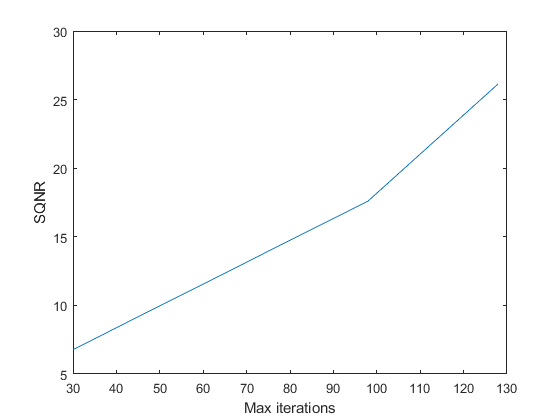
\includegraphics[scale=0.5]{images/Erotima2_2_a.png}}
                \end{figure}
            \item Στο παρακάτω σχήμα φαίνονται τα SQNR και Kmax που παράγουν οι 2 αλγόριθμοι. Ο αλγόριθμος ομοιόμουρφου κβαντισμού είναι "ανεξάρτητος" από το Kmax και άρα ουσιαστικά απλά είναι το γράφημα μεταξύ SQNR και Ν.
                \begin{figure}[H]
                \makebox[\textwidth][c]{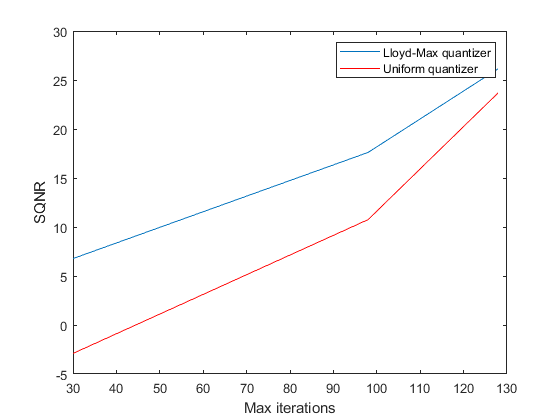
\includegraphics[scale=0.5]{images/Erotima2_2_b.png}}
                \end{figure}
            Για μικρά N, παρατηρούμε αισθητή υπεροχή του Lloyd-Max της τάξης των 10dB που σημαίνει ότι έχει 10 φορές μεγαλύτερη ισχύ σήματος από θόρυβο κβάντισης. Ωστόσο όσο μεγαλώνουν τα N αυτή η απόσταση μεταξύ τους μικραίνει όλο και περισσότερο, με αποτέλεσμα για Ν=6 να έχουμε υπεροχή του Lloyd-Max μόνο κατά 4dB το οποίο ισούται με περίπου 3 φορές μεγαλύτερη ισχύ σήματος από θόρυβο κβάντισης. Όπως εξηγούμε και στο ερώτημα με το MSE παρακάτω, παρατηρούμε ότι για μεγαλύτερα Ν θα υπάρχει μια όλο και πιο έντονη σύγκλιση των δύο αλγορίθμων.  
            \item Υποθέτουμε πως ο κβαντιστής στον οποίο αναφέρεται η εκφώνηση να υπολογίσουμε της πιθανότητα κάθε στάθμης είναι ο ομοιόμορφος όπως διατυπώθηκε από τους βοηθούς κατά τη διάρκεια των βοηθητικών ωρών. Έτσι, αφού ο ομοιόμορφος κβαντιστής ακολουθεί την ομοιόμορφη κατανομή και έχουμε $2^N$ επίπεδα μεγέθους $\Delta$ τότε είναι βέλτιστος όταν η πιθανότητα εμφάνισης κάθε επιπέδου είναι $\dfrac{1}{2^N}$. Ωστόσο, από τα παρακάτω σχήματα αλλά και μετά από μερικούς πειραματισμούς καταλήξαμε ότι η κατανομή που ακολουθεί η πηγή Β δεν είναι ομοιόμορφη αλλά ακολουθεί μάλλον κατανομή Laplace ή Student's γι' αυτό και ο ομοιόμορφος κβαντιστής έχει χαμηλή αποδοτικότητα σε σχέση με τον Lloyd-Max. Ωστόσο, η Laplace δεν υπάρχει ενσωματωμένη στην Matlab και αποφασίσαμε να χρησιμοποιήσουμε την Student's.\\
            Οι πρακτικές και οι θεωρητικές μετρήσεις που έγιναν στον ομοιόμορφο κβαντιστή φαίνονται στα παρακάτω σχήματα  για Ν=2, 4 και 6 bits αντίστοιχα. Παρατηρούμε σχετικά μικρές προς μεσαίες αποκλείσεις αυτό μπορεί να οφείλεται στο ότι η κατανομή εκτιμήθηκε εμπειρικά.

            \newpage
            
                \begin{figure}[H]
                \makebox[\textwidth][c]{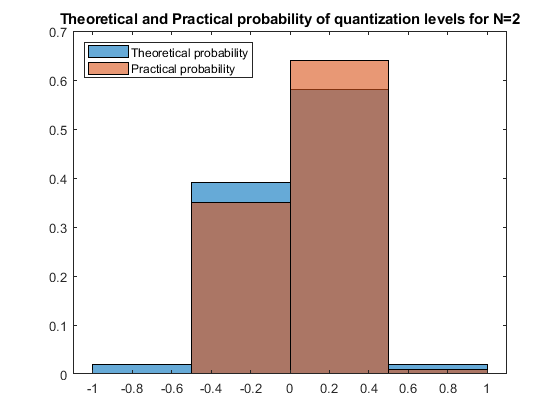
\includegraphics[scale=0.45]{images/Erotima2_2_c_N2_probs.png}}
                \end{figure}
                
                \begin{figure}[H]
                \makebox[\textwidth][c]{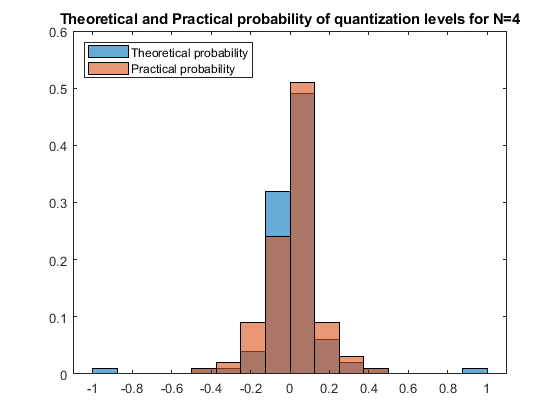
\includegraphics[scale=0.45]{images/Erotima2_2_c_N4_probs.png}}
                \end{figure}
                
                \begin{figure}[H]
                \makebox[\textwidth][c]{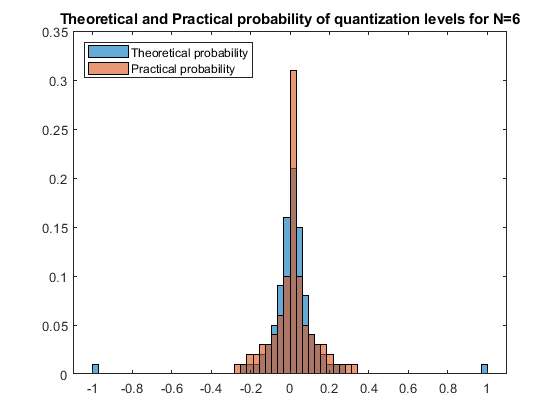
\includegraphics[scale=0.45]{images/Erotima2_2_c_N6_probs.png}}
                \end{figure}
            
            \newpage
            
                Η εντροπία κάθε επιπέδου κβάντισης του ομοιόμορφου κβαντιστή φαίνεται στα παρακάτω σχήματα για Ν=2, 4 και 6 bits αντίστοιχα. Γενικά, παρατηρούμε ότι αυτά τα γραφήματα δεν μας δίνουν κάποια παραπάνω πληροφορία σε σχέση με αυτά των πιθανοτήτων κβάντησης. Αυτό οφείλεται στο ότι η εντροπία είναι η μέση πληροφορία, και έχει νόημα για πηγές όχι για μεμονομένα σύμβολα. Στη περίπτωση των μεμονομένων συμβόλων έχει περισσότερο νόημα η πληροφορία και όχι η εντροπία. Το μόνο που παρατηρούμε είναι ότι παρατηρούμε οι κατανομές να "ανοίγουν" δηλαδή να αυξάνεται η διασπορά τους.
                
                \begin{figure}[H]
                \makebox[\textwidth][c]{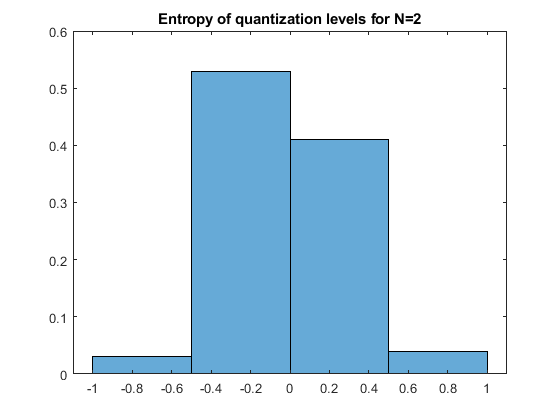
\includegraphics[scale=0.45]{images/Erotima2_2_c_N2_entropy.png}}
                \end{figure}
                
                \begin{figure}[H]
                \makebox[\textwidth][c]{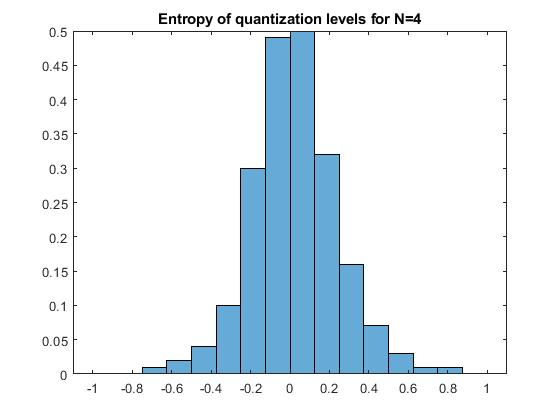
\includegraphics[scale=0.45]{images/Erotima2_2_c_N4_entropy.png}}
                \end{figure}
                
                \begin{figure}[H]
                \makebox[\textwidth][c]{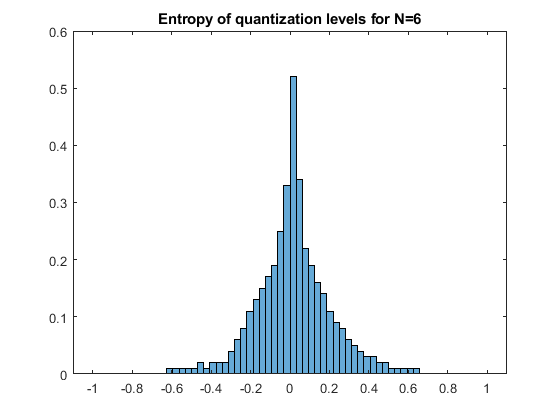
\includegraphics[scale=0.45]{images/Erotima2_2_c_N6_entropy.png}}
                \end{figure}
            
            \item Η αποδοτικοτητά και των δύο κβαντιστών σε σχέση με το MSE παρουσιάζεται παρακάτω. Παρατηρούμε πως ο κβαντιστής Lloyd-Max συγκλίνει πολύ γρηγορότερα το οποίο είναι αναμενόμενο λόγω της φύσης του να προσαρμόζει την κατανομή των επιπέδων κβάντισης του στην κατανομή των δειγμάτων. Ωστόσο παρατηρούμε ότι από Ν=4 και μετά ξεκινάει να υπάρχει ένας κορεσμός οποίος ολοκληρώνεται για Ν=6 και προφανώς για μεγαλύτερα Ν οι δύο κβαντιστές θα συγκλίνουν στο ίδιο MSE. Δηλαδή για Ν=6 και μετά ο ομοιόμορφος κβαντιστής έχει σχεδόν την ίδα απόδοση με τον Lloyd-Max. Αυτό είναι πολύ λογικό αν και στη συγκεκριμένη περίπτωση είναι αισθητό για σχετικά μικρό Ν, είναι αναμενόμενο να συμβεί αφού ο ομοιόμορφος κβαντιστής στην οριακή περίπτωση με άπειρα διαστήματα κβάντισης θα τείνει να έχει την ίδια απόδοση με κάποιον που ακολουθεί μια διαφορετική κατανομή.
                \begin{figure}[H]
                \makebox[\textwidth][c]{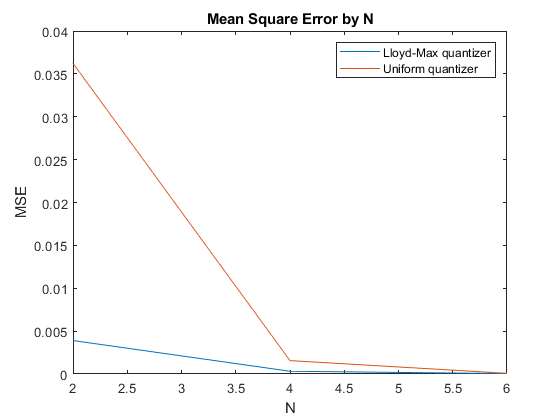
\includegraphics[scale=0.45]{images/Erotima2_2_d.png}}
                \end{figure}
        \end{enumerate}
    \end{enumerate}

\newpage

\section{Ερώτημα 3}

\begin{enumerate}
    \item Με βάση τις παραπάνω υποδείξεις, υλοποιήστε το σύστημα Μ-PΑΜ και
    αναφερθείτε στα βασικά του σημεία.
    \item Μετρήστε την πιθανότητα σφάλματος bit και σχεδιάστε την καμπύλη
    BER για Μ = 2, 4, 8, 16 για απλή κωδικοποίηση για τιμές του SNR =
    0: 5: 40dB . Επαναλάβετε το ερώτημα για Μ = 4, 8, 16 αν τα σύμβολα στην
    αντιστοίχιση κωδικοποιούνταν κατά Gray. Οι καμπύλες να σχεδιαστούν
    όλες στο ίδιο γράφημα.
    \item Μετρήστε την πιθανότητα σφάλματος συμβόλου και σχεδιάστε την
    καμπύλη SER για M = 4, 8, 16 για απλή και κατά Gray κωδικοποίηση για
    τιμές του SNR = 0: 5: 40dB. Οι καμπύλες θα πρέπει και πάλι να
    σχεδιαστούν όλες στο ίδιο γράφημα.
\end{enumerate}

\subsection*{Απάντηση στο Ερώτημα 3}
    \begin{enumerate}
    \item
    Το σύστημα PAM υλοποιήθηκε σύμφωνα με την εκφώνηση. Ο πομπός αποτελείτε από τον Mapper που αντιστοιχεί τα bits σε σύμβολα ώστε ανάλογα με τον τύπο της κωδικοποίησης να μπορούμε να μεταφέρουμε πληροφορία παραπάνω του ενός bit μέσω ενός συμβόλου. Δηλαδή αν έχουμε M=2, έχουμε 4 πιθανά πλάτη του παλμού $g_T(t)$ και άρα μπορούμε να μεταφέρουμε πληροφορία 2 bits σε κάθε παλμό. Ο πομπός περιέχει επίσης και τον Διαμορφωτή που αντιστοιχεί το κάθε σύμβολο σε ένα σήμα εξόδου που σε πραγματική υλοποίηση θα ήταν συνεχές. Ουσιαστικά ο διαμορφωτής εκφράζει το σύμβολο ως ένα διάνυσμα σε έναν χώρο σημάτων, που έχει ως βάση σήματα τα οποία γνωρίζουν ο πομπός  και ο δέκτης. Στην βάση σημάτων αυτή ο πομπός και ο δέκτης, εκ των προτέρων έχουν δημιουργήσει διανυσματα τα οποία αντιστοιχούν σε σύμβολα και την αντιστοίχηση αυτή την γνωρίζουν και οι δύο. Αυτή ονομάζεται αστερισμός. Στη περίπτωση του PAM αυτό ο χώρος σημάτων είναι μονοδιάστατος και έχει ως βάση το $\psi(t) = \dfrac{g_T(t)}{\sqrt E_g}$ και συντελεστές $s_m = \sqrt E_g A_m$. Έτσι, ο δέκτης πολλαπλασιάζει το κάθε σύμβολο με έναν παλμό $g_T(t)$ και στην συνέχεια το πολλαπλασιάζει με το φέρον σήμα $cos(2\pi f_C t)$, ώστε να το μεταφέρει στο επιθυμητό εύρος συχνοτήτων. Ωστόσο στη συγκεκριμένη περίπτωση δεν είναι ιδιαίτερα χρήσιμο καθώς ο ορθογώνιος παλμός έχει άπειρο έυρος συχνοτήτων. Το Κανάλι εισάγει προσθετικό λευκό θόρυβο κανονικής κατανομής (AWGN) και μοντελοποιεί τον θόρυβο που εισάγεται από τα ηλεκτρονικά του δέκτη. Ο δέκτης αποτελείτε από τον Αποδιαμορφωτή, τον Φωρατή και τον Demapper. O αποδιαμορφωτής αντιστρέφει τη λειτουργία του διαμορφωτή, ουσιαστικά δρα σαν χαμηλοπερατό φίλτρο αφαιρόντας την συχνότητα του φέροντος σήματος από το φάσμα συχνοτήτων του ληφθέντος σήματος και στη συνέχεια αφαιρεί και τη DC συνιστώσα, που δεν υπάρχει στη περίπτωση μας. Ο φωρατής λαμβάνει αποφάσεις σχετικά με το ποιο σύμβολο αντιστοιχεί σε κάθε τιμή του αποδιαμορφωτή και ο Demapper αντιστοιχίζει σύμβολα σε bits. Ουσιαστικά, στην γενική περίπτωση, ο φορατής λαμβάνει ένα διάνυσμα σήματος που είναι το στιγμιότυπο μιας τυχαίας διαδικασίας AWGN το οποίο ανήκει πιθανότατα σε χώρο σημάτων μεγαλύτερης διάστασης από την γνωστή βάση σημάτων στην οποία επικοινωνεί με τον δέκτη. Αυτό το διάνυσμα καλείται να το προβάλει στη γνωστή βάση αυτή και να επιλέξει σε ποιο διάνυσμα του αστερισμού βρίσκεται κοντινότερα, μέσω τις Ευκλείδιας απόστασης.
    
    Στην υλοποίηση μας η κάθε μονάδα λειτουργεί ως εξής:
    \begin{itemize}
        \item Mapper \\
        Παίρνει ως είσοδο ένα διάνυσμα από bits μεγέθους $K\times1$, το μετατρέπει σε ένα πίνακα $\dfrac{K}{M}\times M$ και στη συνέχεια σε κάθε γραμμή έχουμε ένα δυαδικό αριθμό τον οποίο τον μετατρέπουμε σε δεκαδικό. Στη περίπτωση της κωδικοποίησης Gray σε αυτό το σημείο μετατρέπουμε τα ακέραια στοιχεία σε κωδικοποιημένα κατά Gray στοιχεία. Στη συνέχεια αντιστοιχίζεται στο κατάλληλο πλάτος $s_m$ του αστερισμού.
        \item Διαμορφωτή \\
        Από την εκφώνηση γνωρίζουμε ότι έχουμε 40 δείγματα ανά μεταδιδόμενο σύμβολο και ότι η περίοδος κάθε συμβόλου περιλαμβάνει 10 κύκλους φέρουσας. Η έξοδος του διαμορφωτή για την χρονική διάρκεια μιας περιόδου ενός συμβόλου δίνεται από τον τύπο (2) της εκφώνησης. Ουσιαστικά επειδή το $g_T(t)$ είναι ορθογώνιος παλμός, κάθε περίοδος συμβόλου αποτελείται από 10 συνημιτονικούς παλμούς πολλαπλασιασμένους με το πλάτος που επιλέχθηκε στον Mapper. Για κάθε έναν από αυτούς τους παλμούς έχω 4 δείγματα. Σε ένα διάνυσμα όλες αυτές οι τιμές είναι το διάνυσμα εξόδου από τον πομπό.
        \item Κανάλι με AWGN \\
        Στο σημείο αυτό υπολογίζεται ο θόρυβος και εισάγεται στο σήμα εξόδου σύμφωνα με την εκφώνηση.
        \item Αποδιαμορφωτής \\
        Λαμβάνει ως είσοδο το διάνυσμα του σήματος από το κανάλι. Το πολλαπλασιάζει με το φέρον σήμα και στη συνέχεια αθροίζει/ολοκληρώνει τις τιμές κάθε συμβόλου. Έτσι παίρνουμε ως έξοδο ένα διάνυσμα με μέγεθος ίσο με τον αριθμό των συμβόλων που εκπέμφθηκαν αλλά επειδή στο κάθε σύμβολο έχει εισαχθεί θόρυβος πρέπει να αποφασίσουμε σε ποιό πλάτος του αστερισμού θα αντιστοιχήσουμε το καθένα.
        \item Φορατής \\
        Αντιστοιχίζει κάθε σημείο του διανύσματος που έλαβε στο κοντινότερο σημείο με βάση την Εκλείδια απόσταση σημείο από τον αστερισμό της κωδικοποίησης. Μετά μέσω του αντίστροφου αστερισμού αντιστοιχεί το κάθε πλάτος αστερισμό στο αρχικό του σύμβολο.
        \item Demapper \\
        Αντιστρέφει τη λειτουργία του Mapper. Στην περίπτωση της κωδικοποίσης κατά Gray εκτελεί την επιπλέον πράξη της αποκωδικοποίησης του διανύσματος των ακεραίων. Τέλος, αντιστοιχίζει κάθε δεκαδικό σύμβολο στα bits στα bits της δυαδική του αναπαράστασης και φτιάχνει ένα διάνυσμα με τα bits των συμβόλων.
    \end{itemize}
    
    Στα παρακάτω σχήματα παρουσιάζεται η λειτουργία του ψηφιακού συστήματος.
        \begin{figure}[H]
        \makebox[\textwidth][c]{
        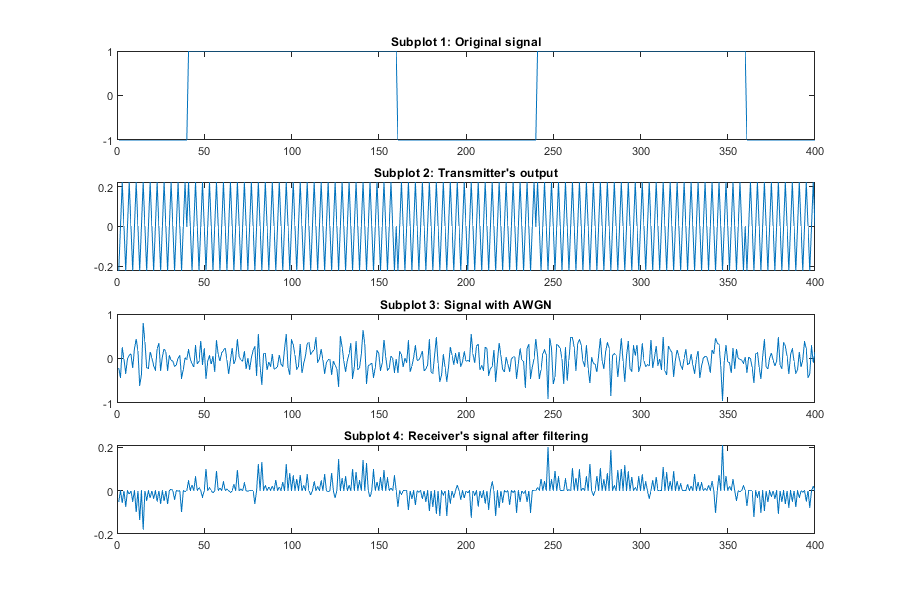
\includegraphics[scale=0.40]{images/M2_SNR10_1.png}}
        \caption{Προσομοίωση PAM δυαδικής κωδικοποίησης με M = 2 και SNR = 10dB}
        \end{figure}
        \begin{figure}[H]
        \makebox[\textwidth][c]{
        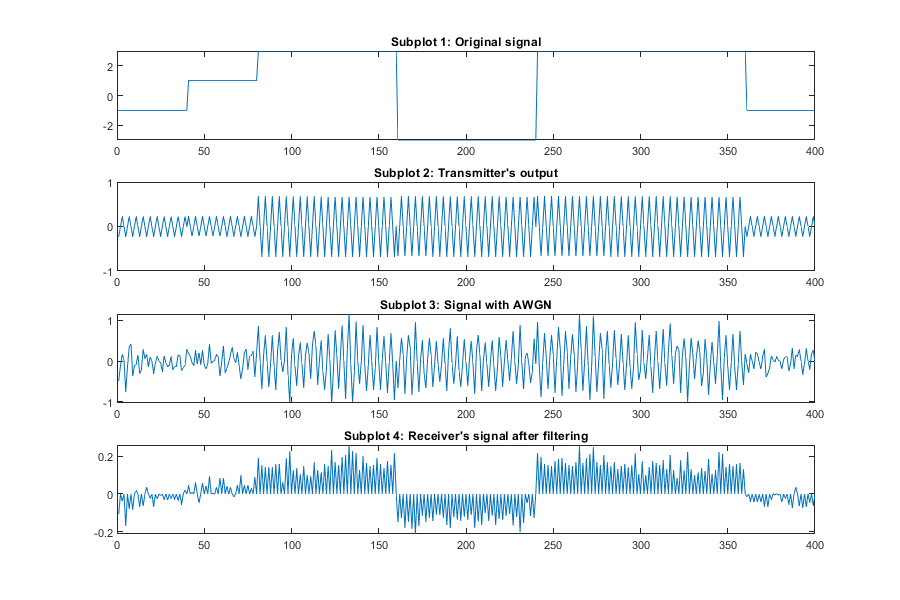
\includegraphics[scale=0.40]{images/M4_SNR10_1.png}}
        \caption{Προσομοίωση PAM δυαδικής κωδικοποίησης με M = 4 και SNR = 10dB}
        \end{figure}
        \begin{figure}[H]
        \makebox[\textwidth][c]{
        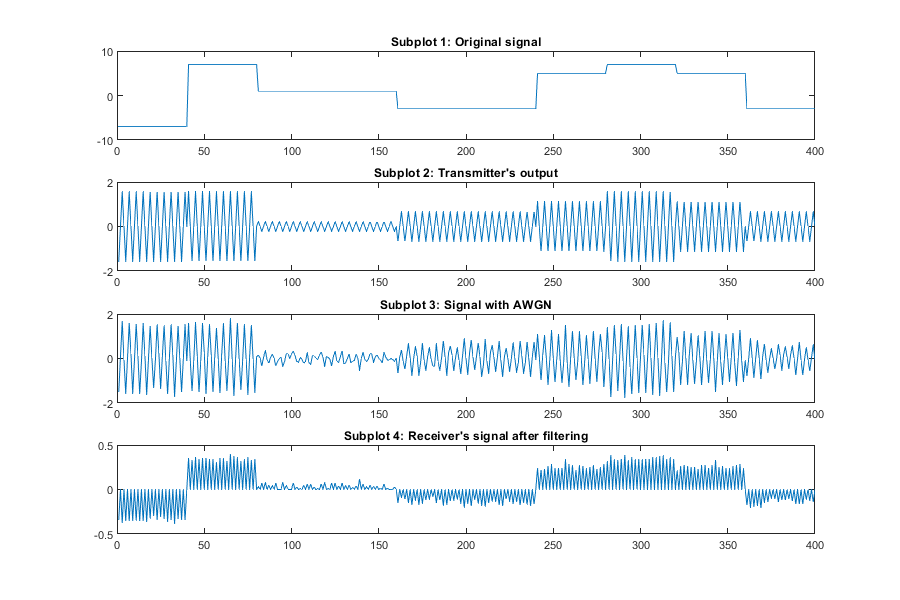
\includegraphics[scale=0.40]{images/M8_SNR10_1.png}}
        \caption{Προσομοίωση PAM δυαδικής κωδικοποίησης με M = 8 και SNR = 10dB}
        \end{figure}
        \begin{figure}[H]
        \makebox[\textwidth][c]{
        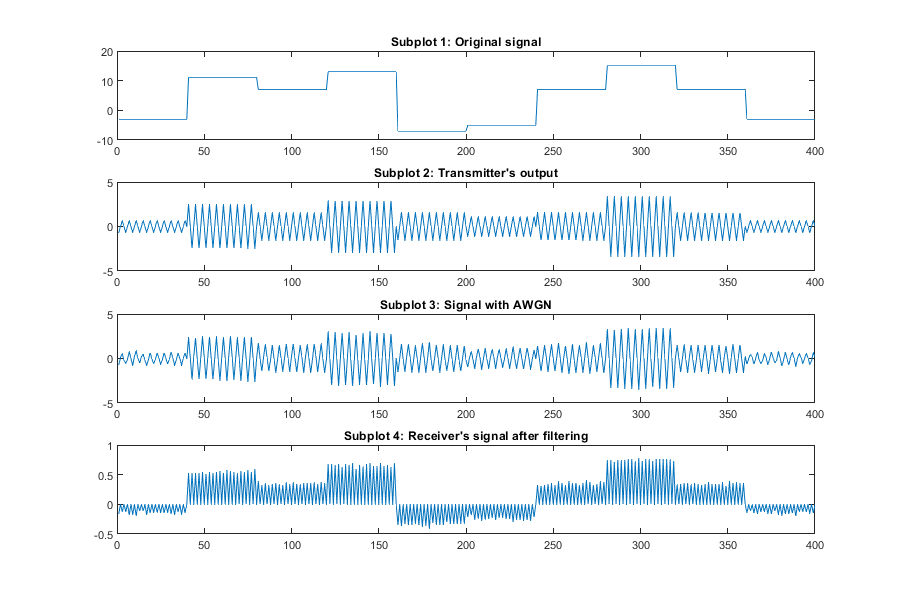
\includegraphics[scale=0.40]{images/M16_SNR10_1.png}}
        \caption{Προσομοίωση PAM δυαδικής κωδικοποίησης με M = 16 και SNR = 10dB}
        \end{figure}
    \item 
        Γενικές παρατηρήσεις στις καμπύλες BER/SER :
        \begin{itemize}
            \item Για σταθερό SNR το BER/SER μειώνεται όσο αυξάνεται το M, το οποίο είναι λογικό αφού ο AWGN του καναλιού μας είναι αντιστρόφως ανάλογος του $\log_2(M)$.
            \item Για σταθερό M το BER/SER μειώνεται όσο αυξάνεται το SNR, το οποίο είναι απολύτως λογικό αφού μειώνεται ο θόρυβος που εισάγεται από το κανάλι και είναι πιο εύκολη η κωδικοποίηση.
            \item Στην περίπτωση της κωδικοποίησης Gray έχουμε αισθητή διαφορά στο BER, το οποίο είναι αναμενόμενο. Γνωρίζουμε ότι κατά την αποκωδικοποίηση λόγω της κατανομής του Gaussian θορύβου με μέση τιμή 0 είναι πολύ πιο πιθανό ένα σύμβολο να αποκωδικοποιηθεί λάθος ως κάποιο γειτονικό του παρά ως κάποιο πιο μακρινό. Έτσι στη περίπτωση που έχουμε κάποιο σφάλμα συμβόλου έχουμε τα ελάχιστα bit σφάλματος. Ωστόσο δεν ισχύει η ίδια αιθητή βελτίωση στη περίπτωση του SER, αφού αυτό εξαρτάται μόνο από την κατανομή του θορύβου.
        \end{itemize}
        
        Στα παρακάτω σχήματα παρουσιάζονται οι ΒER για τις ζητούμενες διαμορφώσεις του PAM.

        \begin{figure}[H]
        \makebox[\textwidth][c]{
        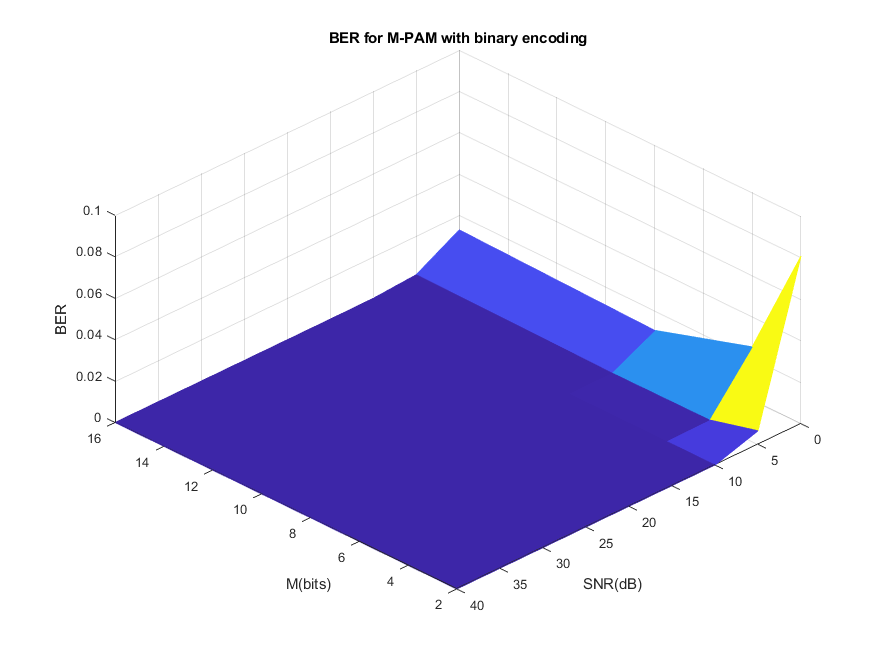
\includegraphics[scale=0.40]{images/BER_Binary.png}}
        \caption{Καμπύλη BER για δυαδική κωδικοποίηση, M = [2, 4, 8, 16] bits και SNR = 0:5:40dB}
        \end{figure}
        \begin{figure}[H]
        \makebox[\textwidth][c]{
        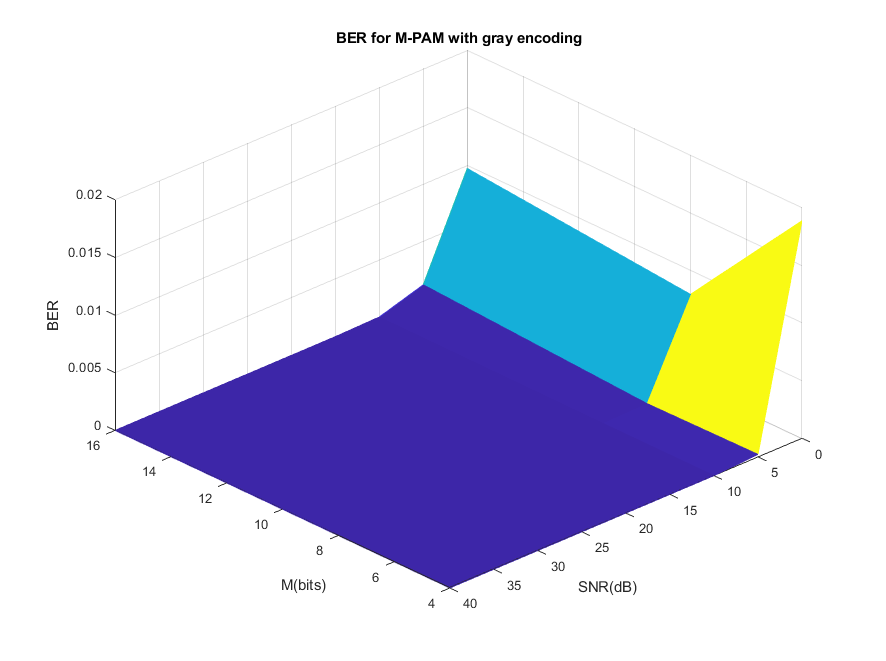
\includegraphics[scale=0.40]{images/BER_Gray.png}}
        \caption{Καμπύλη BER για κωδικοποίηση Gray, M = [4, 8, 16] bits και SNR = 0:5:40dB}
        \end{figure}
        
    \newpage 
    
    \item Στα παρακάτω σχήματα παρουσιάζονται οι SER για τις ζητούμενες διαμορφώσεις του PAM.
        \begin{figure}[H]
        \makebox[\textwidth][c]{
        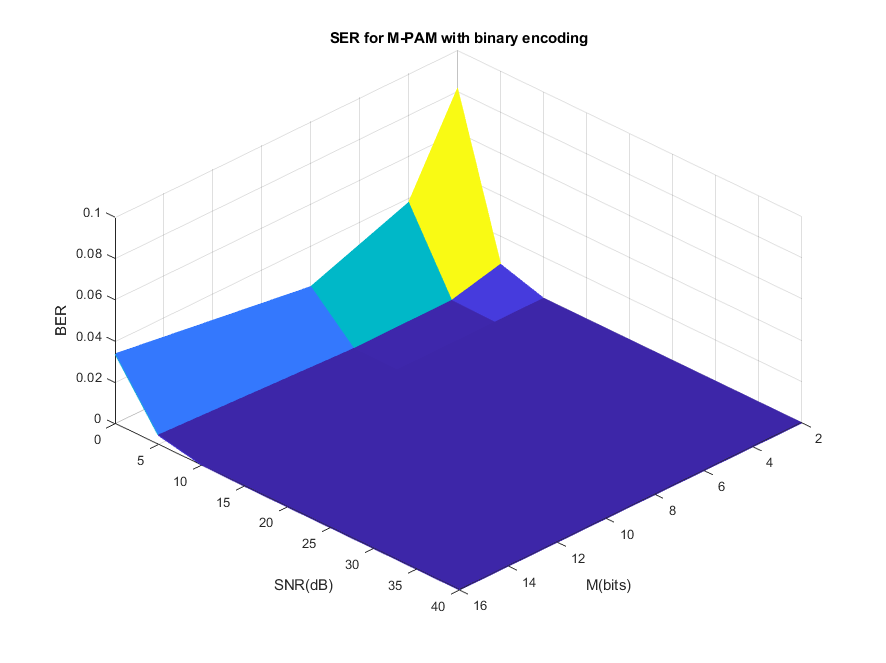
\includegraphics[scale=0.40]{images/SER_Binary.png}}
        \caption{Καμπύλη SER για δυαδική κωδικοποίηση, M = [2, 4, 8, 16] bits και SNR = 0:5:40dB}
        \end{figure}
        \begin{figure}[H]
        \makebox[\textwidth][c]{
        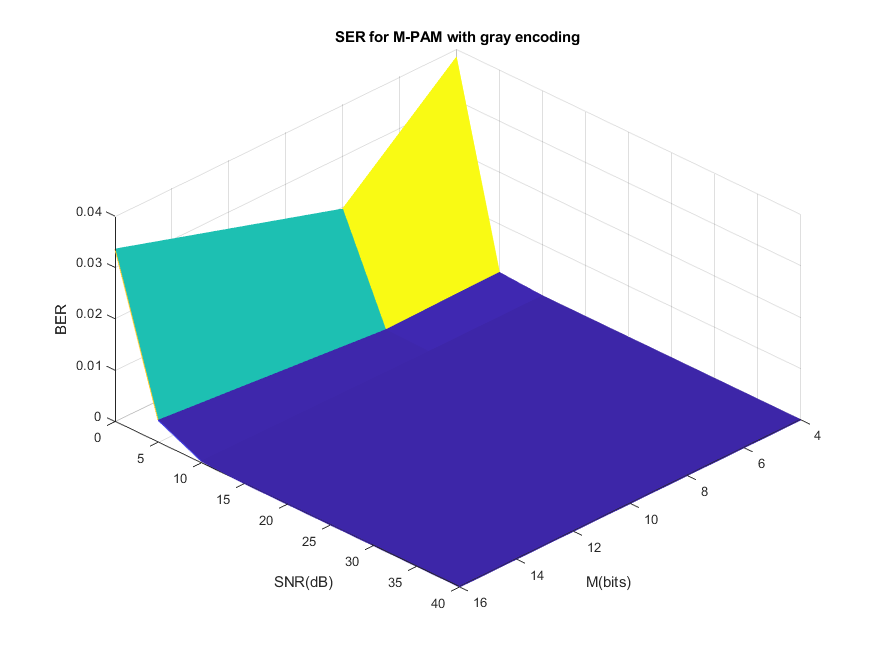
\includegraphics[scale=0.40]{images/SER_Gray.png}}
        \caption{Καμπύλη SER για κωδικοποίηση Gray, M = [4, 8, 16] bits και SNR = 0:5:40dB}
        \end{figure}
    \end{enumerate}

\newpage

\section{Κώδικας}
    \lstinputlisting[caption={Πηγαίος κώδικας για \textsf{Erotima\_1\_2.m}}, captionpos=b]
    {code/Erotima_1/Erotima_1_2.m}
    \lstinputlisting[caption={Πηγαίος κώδικας για \textsf{Erotima\_1\_3.m}}, captionpos=b]
    {code/Erotima_1/Erotima_1_3.m}
    \lstinputlisting[caption={Πηγαίος κώδικας για \textsf{Erotima\_1\_4.m}}, captionpos=b]
    {code/Erotima_1/Erotima_1_4.m}
    \lstinputlisting[caption={Πηγαίος κώδικας για \textsf{Erotima\_1\_5.m}}, captionpos=b]
    {code/Erotima_1/Erotima_1_5.m}
    \lstinputlisting[caption={Πηγαίος κώδικας για \textsf{huffmandict1.m}}, captionpos=b]
    {code/Erotima_1/huffmandict1.m}
    \lstinputlisting[caption={Πηγαίος κώδικας για \textsf{huffmanenco1.m}}, captionpos=b]
    {code/Erotima_1/huffmanenco1.m}
    \lstinputlisting[caption={Πηγαίος κώδικας για \textsf{huffmandeco1.m}}, captionpos=b]
    {code/Erotima_1/huffmandeco1.m}
    
    \lstinputlisting[caption={Πηγαίος κώδικας για \textsf{Lloyd\_Max.m}}, captionpos=b]
    {code/Erotima_2/Lloyd_Max.m}
    \lstinputlisting[caption={Πηγαίος κώδικας για \textsf{my\_quantizer.m}}, captionpos=b]
    {code/Erotima_2/my_quantizer.m}
    \lstinputlisting[caption={Πηγαίος κώδικας για \textsf{quantization\_theoretical_probs.m}}, captionpos=b]
    {code/Erotima_2/quantization_theoretical_probs.m}
    \lstinputlisting[caption={Πηγαίος κώδικας για \textsf{Erotima\_2\_1\_a.m}}, captionpos=b]
    {code/Erotima_2/Erotima_2_1_a.m}
    \lstinputlisting[caption={Πηγαίος κώδικας για \textsf{Erotima\_2\_2\_a.m}}, captionpos=b]
    {code/Erotima_2/Erotima_2_2_a.m}
    \lstinputlisting[caption={Πηγαίος κώδικας για \textsf{Erotima\_2\_2\_b.m}}, captionpos=b]
    {code/Erotima_2/Erotima_2_2_b.m}
    \lstinputlisting[caption={Πηγαίος κώδικας για \textsf{Erotima\_2\_2\_c.m}}, captionpos=b]
    {code/Erotima_2/Erotima_2_2_c.m}
    \lstinputlisting[caption={Πηγαίος κώδικας για \textsf{Erotima\_2\_2\_d.m}}, captionpos=b]
    {code/Erotima_2/Erotima_2_2_d.m}
    
    \lstinputlisting[caption={Πηγαίος κώδικας για \textsf{M\_PAM.m}}, captionpos=b]
    {code/Erotima_3/M_PAM.m}
    \lstinputlisting[caption={Πηγαίος κώδικας για \textsf{Erotima\_3\_b.m}}, captionpos=b]
    {code/Erotima_3/Erotima_3_b.m}
    \lstinputlisting[caption={Πηγαίος κώδικας για \textsf{Erotima\_3\_c.m}}, captionpos=b]
    {code/Erotima_3/Erotima_3_c.m}
\end{document}